\documentclass[12pt]{article}
\usepackage{amsmath,mathtools}
\usepackage[usenames,dvipsnames]{xcolor}
%\usepackage[bitstream-charter]{mathdesign}
%\usepackage{mathptmx}

\usepackage{textcomp}
\usepackage{cmbright}
\usepackage[ngerman]{babel}
\usepackage{microtype}
%\usepackage{microtype}
\usepackage[utf8]{inputenc}
\usepackage[T1]{fontenc}
\usepackage{helvet}
\renewcommand{\familydefault}{\sfdefault}

\usepackage{siunitx}
%\usepackage{tikz}
\usepackage{fancyhdr}
\usepackage{sectsty}
\usepackage{setspace}
\usepackage{booktabs} % To thicken table lines
\usepackage[version=4]{mhchem}
\usepackage{textcomp}
%\usepackage[compatibility=4.7,language=german]{chemmacros}
\usepackage{tabulary}

\usepackage[ddmmyyyy]{datetime}
\renewcommand{\dateseparator}{.}

\pagestyle{fancy}

\cfoot{\thepage}

\lhead{Nevroz Arslan }
\rhead{\today}
\setlength{\headheight}{15pt}

\usepackage{overcite}
\renewcommand\citeform[1]{[#1]}

%\renewcommand*\printatom[1]{{\fontsize{10}{12}\selectfont\ensuremath{\mathsf{#1}}}}
\sectionfont{\fontsize{12}{15}\selectfont}

\makeatletter
    \setlength\@fptop{0\p@}
\makeatother


\newcommand\textbox[1]{%
  \parbox{.333\textwidth}{#1}%
}


\setlength{\headheight}{15pt}
\sisetup{detect-weight=true, detect-all}
\sisetup{text-celsius = $^\circ\mkern-1mu$C}


\renewcommand{\thesection}{\arabic{section}.}
\renewcommand{\thesubsection}{\thesection\arabic{subsection}}
\renewcommand{\headrulewidth}{0pt}

\begin{document}
%%%%%%%%%%%%%
\begin{onehalfspace}

\begingroup
\leftskip=0cm plus 0.5fil \rightskip=0cm plus -0.5fil
\parfillskip=0cm plus 1fil
 \textbf{\large Darstellung von 2-(1\textit{H}-Inden-1-yl)acetaldehyd}\par
\endgroup
\begin{center}
 \textbf{Präparat Nr. 7 von 7}
\end{center}
\section{Reaktionstyp: \textnormal{Iod-Katalysierte Acetalspaltung} }
\begin{figure}[ht]
\centering
\includegraphics[scale=0.25]{reaktion.png}
\end{figure}

\section{Berechnung des Ansatzes: }
Es sollte 2-(1\textit{H}-Inden-1-yl)acetaldehyd aus 1-(2,2-Diethoxyethyl)-1\textit{H}-inden (14.81 \si{\gram}, 63.8 \si{\milli\mol}) hergestellt werden. Die Umrechnung des Literaturansatzes ergab folgenden Ansatz:\cite{vor}\\\\
\noindent
\begin{tabulary}{\textwidth}{Ccccc}
\toprule
\textbf{ Bezeichnung }&\textbf{M [\si{\gram\per\mol}]} & \textbf{ n [\si{\milli\mol}]} & \textbf{Menge}&  \textbf{Equiv}\\
\midrule
 1-(2,2-Diethoxyethyl)-1\textit{H}-inden         & 232.15   & 63.8  & 14.81 \si{\gram} & 1.00 \\
 Iod                                             & 253.18   & 6.4  & 1.62  \si{\gram} & 0.10 \\
 Aceton &   &  & 1000 \si{\milli\liter} & LM \\
\bottomrule
\end{tabulary}\\

%%%%%%%%%%%%%
% Durchführung
%%%%%%%%%%%%%
\section{Durchführung:\cite{vor}}
In einem 2000 \si{\milli\liter} Rundkolben, ausgestattet mit Rückflusskühler und Kontaktthermometer, wurde Aceton vorgelegt und auf 40 \si{\celsius} erwärmt. Anschließend wurden 1-(2,2-Diethoxyethyl)-1\textit{H}-inden (14.81 \si{\gram}, 63.8 \si{\milli\mol}) und Iod (1.62 \si{\gram}, 6.4 \si{\milli\mol}) zugegeben und zwei Stunden bei 40 \si{\celsius} gerührt. Danach wurde Natriumthiosulfatlösung (5 \%-ig, 500 \si{\milli\liter}) hinzugegeben und weitere 15 Minuten bei Raumtemperatur gerührt. Das Acetone wurde im Rotationsverdampfer entfernt und MTBE (500 \si{\milli\liter}) hinzugegeben. Die organische Phase wurde abgetrennt. Die wässrige Phase wurde mit MTBE (150 \si{\milli\liter}) extrahiert. Die vereinten organischen Phasen wurden mit einer Kochsalzlösung (gesättigt, 150 \si{\milli\liter}) gewaschen, über Magnesiumsulfat getrocknet und das Lösungsmittel im Rotationsverdampfer entfernt. Das Rohprodukt wurde säulenchromatographisch (\ce{SiO_2}, PE/MTBE = 19:1 $\rightarrow$ 1:1) gereinigt und anschließend im Vakuum bei einer Kopftemperatur von 71 \si{\celsius} bei 0.05 \si{\milli\bar} fraktioniert destilliert. Das Produkt (3.15 \si{\gram}, 20.0 \si{\milli\mol}, 34 \%) wurde als gelbe Flüssigkeit erhalten.
%%%%%%%%%%%%
% Ausbeute
%%%%%%%%%%%%%
\section{Ausbeute:}
\begin{tabular}{ ll}
  10.09 \si{\gram} (63.8 \si{\milli\mol})   & = 100 \%\\
  3.15 \si{\gram} (20.0 \si{\milli\mol})   & = 34 \% (Lit.:\cite{vor} 58 \%) \\
 \end{tabular}
\newpage 
\section{Spektrenauswertung:}
\begin{figure}[!htbp]
   \centering
\includegraphics[scale=0.3]{auswert.png}
\end{figure}
\noindent
\textbf{\ce{^1_{}H-NMR}} (500 MHz, \ce{CDCl_3}): \sffamily \ce{$\delta$} =
2.67 (ddd, \ce{^2_{}\textit{J}} = 17.6 \si{\hertz}, \ce{^3_{}\textit{J}} = 7.9 \si{\hertz}, \ce{^3_{}\textit{J}} = 1.5 \si{\hertz}, 1 H, 2-H),
2.91 (ddd, \ce{^2_{}\textit{J}} = 17.6 \si{\hertz}, \ce{^3_{}\textit{J}} = 5.9 \si{\hertz}, \ce{^3_{}\textit{J}} = 1.5 \si{\hertz}, 1~H, 2-H), 
3.92 - 3.97 (m, 1 H, 3-H),
6.54 (dd, \ce{^3_{}\textit{J}} = 5.5 \si{\hertz}, \ce{^3_{}\textit{J}} = 1.9 \si{\hertz}, 1 H, 4-H), 
6.86 (dd, \ce{^3_{}\textit{J}} = 5.5 \si{\hertz}, \ce{^4_{}\textit{J}} = 1.7 \si{\hertz}, 1 H, 5-H), 
7.22 (td, \ce{^3_{}\textit{J}} = 7.4 \si{\hertz}, \ce{^4_{}\textit{J}} = 0.9~\si{\hertz}, 1 H, 7-H),
7.29 (t, \ce{^3_{}\textit{J}} = 7.4 \si{\hertz}, 1 H, 10-H),
7.38 (d, \ce{^3_{}\textit{J}} = 7.4 \si{\hertz}, 1~H, 8-H),
7.41 (d, \ce{^3_{}\textit{J}} = 7.4 \si{\hertz}, 1 H, 9-H),
9.74 (t, \ce{^3_{}\textit{J}} = 1.4 \si{\hertz}, 1 H, 1-H) ppm. \\\\
\noindent
\textbf{\ce{^{13}_{}C-NMR}} (125 MHz, DEPT, \ce{CDCl_3}): \sffamily \ce{$\delta$} =
44.2  (\ce{CH_2}, C-2),
44.8  (\ce{CH}, C-3),
121.3 (\ce{CH}, C-8),
123.0 (\ce{CH}, C-9),
125.2 (\ce{CH}, C-7),
127.0 (\ce{CH}, C-10), 
131.9 (\ce{CH}, C-5), 
137.7 (\ce{CH}, C-4),
144.0 (\ce{C}, C-6),
146.2 (\ce{C}, C-11),
201.0 (\ce{C}, C-1) ppm. 
\section{Mechanismus\cite{bio}:}
Die Entfernung der Acetal-Gruppe verläuft unter der katalytischen Wirkung des Iods (\textbf{2}). 
Im ersten Schritt der Reaktion polarisiert das Iod-Molekül (\textbf{2}) das Aceton (\textbf{1}) unter Abspaltung eines Iodids. Es bildet sich ein Carbokation \textbf{3}. Danach erfolgt der nukleophiler Angriff des Acetals (\textbf{4}) auf den elektropositiven Kohlenstoff des Carbokations \textbf{3}. 
Es entsteht dabei ein Oxonium-Kation \textbf{5}. Anschließend erfolgt ein intramolakularer nukleophiler Angriff an einem dem Sauerstoff benachbarten Kohlenstoffatom der Acetal-Gruppe. Unter Abspaltung des 2,2-Diethoxypropan und der Freisetzung des Katalysators \textbf{2} entsteht der gewünschte Aldehyd \textbf{6}.
\noindent
\begin{figure}[!htbp]
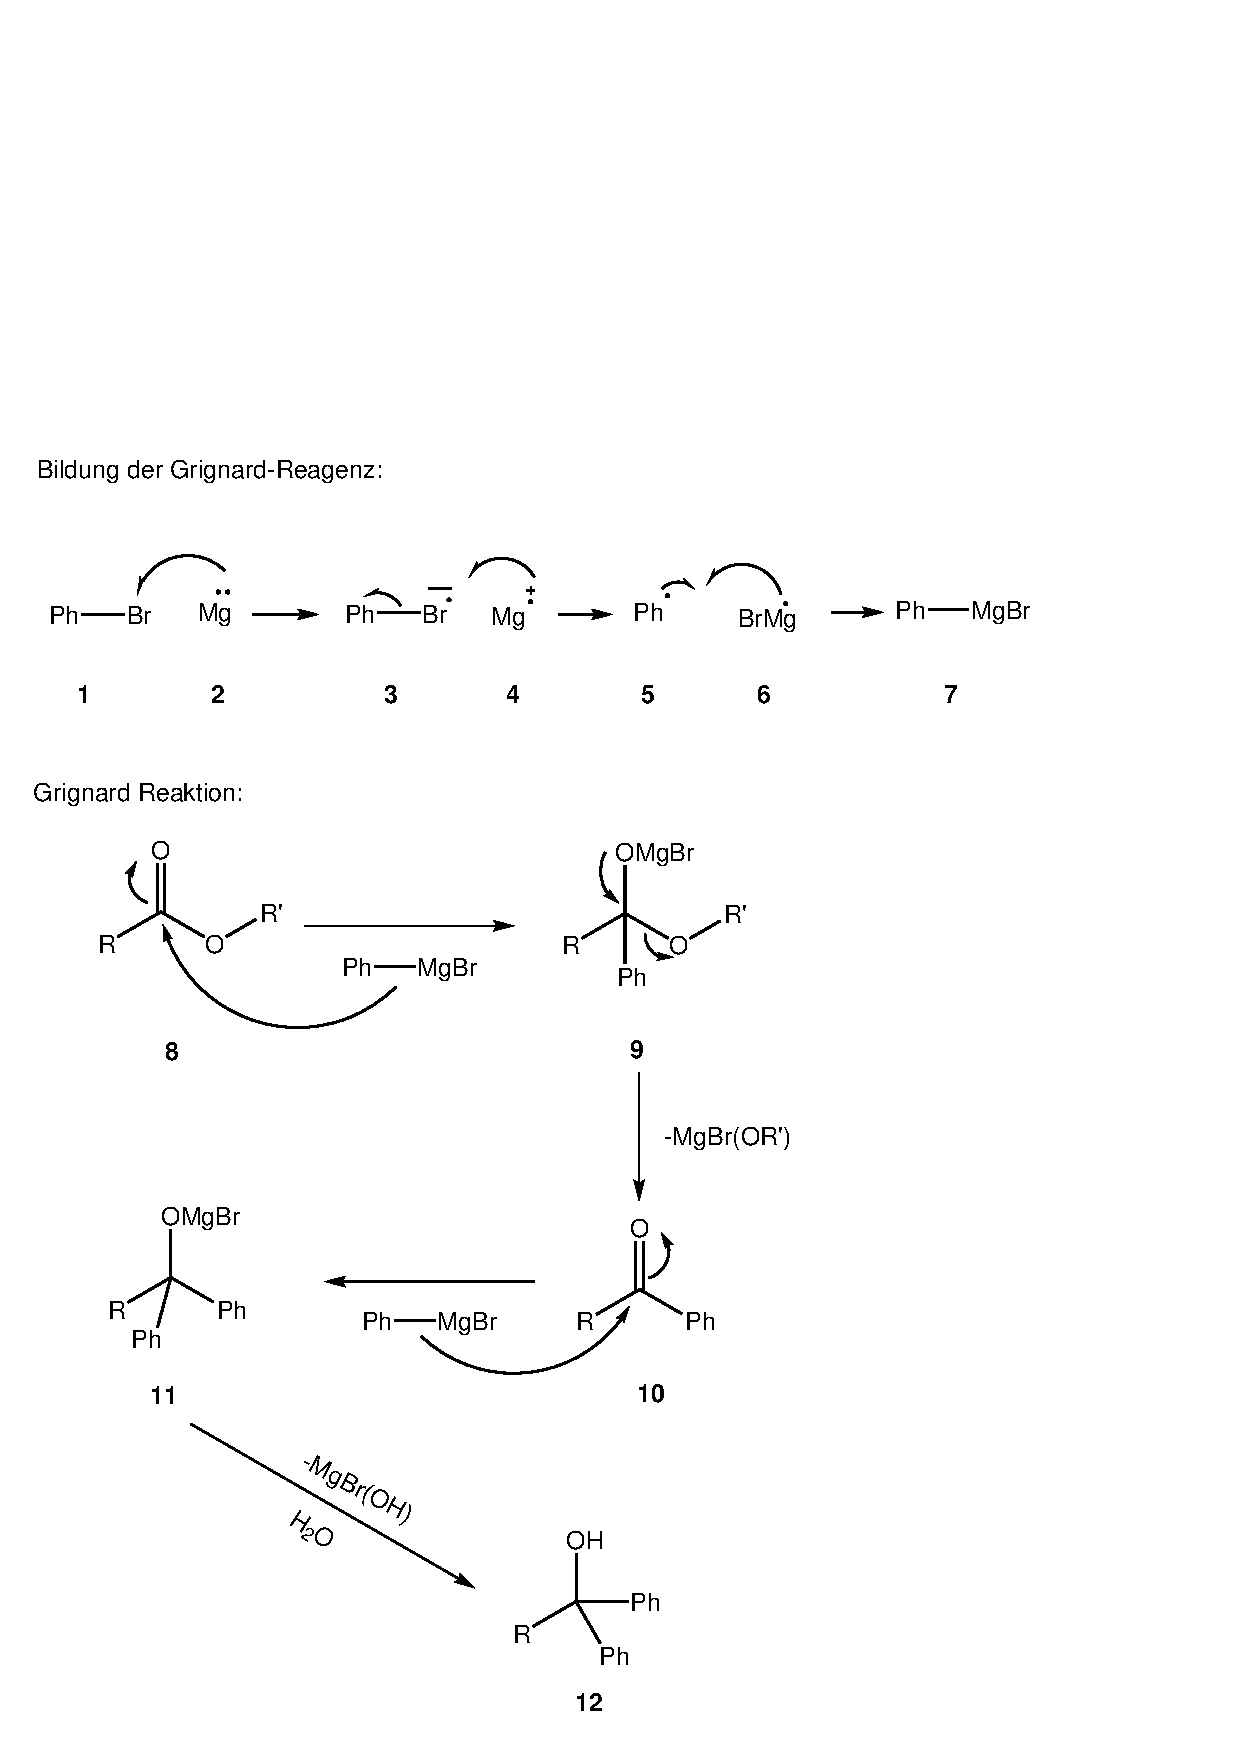
\includegraphics[scale=0.25]{mechan.png}
\end{figure}

\section{Abfallentsorgung:}
Das im Rotationsverdampfer abgetrennte Lösungsmittel wurde im Behälter für halogenfreie Kohlenwasserstoffe entsorgt.
Das nach der Säulenchromatographie abgetrennte Lösungsmittel wurde im Behälter für halogenfreie Kohlenwasserstoffe entsorgt.
Die wässrigen Phasen wurden nach einer pH-Wertbestimmung im Behälter für basische wässrige Abfälle entsorgt.
\section{Literatur:}


\renewcommand{\section}[2]{}%
\def\bibindent{0em}
\begin{thebibliography}{99\kern\bibindent}
\makeatletter
\let\old@biblabel\@biblabel
\def\@biblabel#1{\old@biblabel{#1}\kern\bibindent}
\let\old@bibitem\bibitem
\def\bibitem#1{\old@bibitem{#1}\leavevmode\kern-\bibindent}
\makeatother
\bibitem{vor}
J. H. Ross, S. H. Rohjans, M. Schmidtmann, S. Doye, \textit{Arkivoc} \textbf{2015}, \textit{ii}, 76-92.
\bibitem{bio}
J. Sun, Y. Dong, L. Cao, X. Wang, S. Wang, Y. Hu, \textit{J. Org. Chem.} \textbf{2004}, \textit{69}, 8932-8934.
\end{thebibliography}
\end{onehalfspace}
\end{document}

